\Chapter{Generálás}

- Térkép, úthálózat és egyéb elemek generálása
- Alapelemek megjelenítése HTML Canvas-en.
- Elsősorban gráfokról van szó.

\Section{Úthálózat Generálása}
Maga a generáló algoritmus megalkotásakor első lépésben a nagyvonalakban leírt elvárt működést vizsgáltam. A hálózatnak középponttól kifelé haladva ritkulnia kell, ezzel közelítve egy 
valódi várost. A paraméterezéssel kapcsolatos elvárásokat könnyen meg lehet valósítani. Egy gráfként képzelhető el a megalkotott úthálózat, melynek csomópontjai jelölik az egyes útelemek 
elejét, élei pedig azoknak tartományát. A gráf 0. szintjét jelöltem el a hálózat középpontjának, innen mindig 4 irányba indulnak élek. Minden további csomópont generálódásakor kapja meg 
annak értékét, hogy mennyi irányba indulnak belőle élek. A csomópontok generálása a következőképpen történik:
\begin{enumerate}
\item A kiválasztott csomópont kap egy véletlenszerű irányt, észak, dél, kelet, vagy nyugat értékében
\item Ha a kapott érték megegyezik azzal az iránnyal amerre a csomópont szülője van, vagy már indult arra belőle él, újat kap
\item A kiválasztott iránynak megfelelő véletlen generált X és Y koordinátákat kap
\item A kapott koordinátákból alkotott csomópont felkerül a gráfra
\item Ha a jelenlegi csomópontból még kell éleket indítani, akkor kezdődik előröl
\end{enumerate}
Az előbbiekben említett X és Y koordinátát kissé pontosítanám. Ha a csomópontot nyugat vagy kelet irányba generáljuk, az X koordináta értéke a jelenlegi pont X koordinátája, hozzáadva egy
előre definiált értékek közötti véletlen szám. Az Y koordináta ilyenkor egy minimális eltérés az út fekvésében, hasonlóan generálódik, de lényegesen alacsonabb véletlen számot kap. Ez
tulajdonképpen a valóságban is látható "tökéletlenségekre" vezethető vissza, ugyanis a legtöbb esetben ott sem teljesen merőleges egymásra kettő út. Az észak és dél irányba induló pontok 
esetén ugyan ez az eljárás, csak a két koordináta szerepe felcserélődik.
Fontos viszont az is, hogy a középponttól távolodva átlagosan kevesebb elágazása legyen egy csomópontnak, ezért ehhez felhasználható annak gráfbeli szintje. Minden csomópontról eltárolódik 
annak szintje (szülő szintje + 1), ami befolyásolja az elágazások számát. Egy másik probléma az, hogy az így generált élek gyakran metszhetik egymást, amely az aluljárók és a hídak hiányában 
itt nem megengedett, ezért utolsó lépésnek ellenőrizni kell hogy az új él metszi-e bármely meglévő élek közül akár az egyiket is, és ha igen akkor nem kerülhet fel a gráfra. Az él viszont hozzáadható 
az eredetileg kijelölt csomóponthoz legközelebbi csomóponttal történő helyettesítéssel, feltéve ha így nem történik létező út metszése.
A kanyarok beépítése megoldható azzal, ha az olyan csomópontoknál ahol közel merőlegesen találkozik két él, egy körívet húzunk. A buszmegállók elhelyezésével kapcsolatban a következő feltételeket
adtam:
\begin{itemize}
\item A legcélszerűbb a hálózat két, egymástól távol lévő, a gráf mélyebb szintjein elhelyezkedő pont közötti út létrehozása
\item Az útvonalnak érintenie kell a középpontot, a gráf 0. szintjét
\item Lehető legkevesebbszer érintse többször ugyan azt a csomópontot
\item Ne legyen két megálló két egymás melletti csomóponton
\end{itemize}
Ennek érdekében először kijelölöm az út egyik végét, mint megállót. Ezek után keresek egy utat a gráf 0. szintjéhez, melyen legfeljebb minden második csomópontot kijelölöm megállónak. A középpont 
elérése után kijelölöm a második végpontot, mely a középponttól az eddigi iránynak ellentétesen, a gráf mélyebb szintjei közül kell lennie. Az ehhez a középpontból vezető úton, az utóbbihoz hasonló 
eljárással kijelölök megállókat. Az utak sávszámának meghatározására a gráfbeli mélységüket használom. A magasabb szinten lévő élek nagyobb valószínűséggel lesznek többsávosak. Ez a generálás végén választódik
ki. Az egyirányú utak kijelölése is a folyamat legvégén történik. Ennek az oka magából az utak jellegéből adódik, ugyanis egyirányú út nem végződhet zsákutcában. Éppen ezért egy olyan részgráfot kell találni amely Hamilton-kört 
alkot, amelyen egy részgráfot már nyugodtan egyirányúvá lehet tenni.
\Section{Alapelemek megjelenítése HTML Canvas segítségével}
Az algoritmus működését, eredményét egy HTML Canvas objektumon szemléltetem. Magát a kódot JavaScript-ben írtam, annak ECMAScript 6-os verziójában. Fejlesztői környezetnek A JetBrains által készített WebStormot használtam. Először is 
létrehoztam egy HTML fájlt, ahol a body tag-en belül elhelyeztem a canvas elemet. Erre az elemre JavaScriptből a HTML-ben megadott id-je alapján lehet hivatkozni. Ezután létrehoztam egy JavaScript fájlt, melyben egy (document).ready() szintaktikában 
elhelyezett függvényhívással indítom a generálást. A (document).ready() a jQuery függvénykönyvtárnak része. Azért szükséges ebben az esetben, mert ameddig a html fájl nem töltött be teljesen, a script nem futtatható mert a canvas elemre nem létezne 
semmilyen referencia. Ez a részlet biztosítja hogy csak akkor kezdődjön a script futtatása, ha a HTML documentum teljesen betöltött. Ha ez megtörtént, meghívódik a DrawOnCanvas függvény. Először is ez eltárolja változóként a canvas-ra vonatkozó referenciát.
szintén új változóba, utána a myCanvas.getContext("2d") létrehoz egy CanvasRenderingContext2D objektumot, mellyel a canvasra rajzolni lehet. A következő lépésben megtörténik a paraméterek beállítása, azaz mennyi legyen a maximális csomópontok száma, átlagosan milyen hosszúak legyenek az utak. 
A kontextust elmozdítjuk alapértelmezett helyéről, (0,0)-ról az (1000,500) pontba. Létrehozzuk a kezdő csomópontot ezen a pozíción, és hozzáadjuk a csomópontokat tartalmazó tömbhöz. Létrehozzuk az éleket tartalmazó tömböt, majd kirajzoljuk az első csomópontot, melyet egy négyzettel ábrázolok a kontextus .fillRect() függvényével. 
A többi csomópont generálásához itt egy ciklust indítok, mely addig fog futni ameddig a csomópontokat tartalmazó tömb elemszáma el nem éri a paraméterként megadott értéket. Minden iterációban a csomópontok tömbjéből a következő elemet választja ki első lépésben, a 0-tól indulva. 
A kontextust áthelyezem a jelenlegi csomópont pozíciójába, majd beállítok négy logikai változót, melyek megadják hogy ebből a csomópontból a négy irány közül valamelyikébe mentünk-e már tovább. Kezdetben mindegyik hamis értéket kap. Ezt követően egy switch utasítással megkeresem melyik az az irány ahonnan az adott 
csomópontot kiterjesztettük, és ennek megfelelően arra nem mehet tovább. Akár úgy is lehet venni hogy a jelenlegi pontból arrafelé már "húztunk élet", a logikai változó értéke erre vonatkozóan hamissá válik. Különleges eset a kiindulási pont viszont, 
ahol egyik irányra sem igaz ez, ezért csak szimplán továbbmegy a program. Ezután következik egy újabb ciklus, mely a csomópontból húzandó éleken iterál végig, tehát a kiindulási pontnál 4 alkalommal fog ismétlődni. Legelőször is belép egy végtelen ciklusba, ahonnan csak akkor szabadulhat 
break utasítással, ha a ciklus elején véletlenszerűen kisorsolt irányba húzható él. Ha nem akkor újat sorsol. Ezután egy switch szerkezet következik a direction nevű változóra, mely az előbb kapott irányt tárolja. Észak és dél esetén az új csomópont X koordinátája egy 
előre definiált (minimális) értékek közötti véletlen szám, melyhez hozzáadjuk a jelenlegi pont X koordinátáját. Ez a szám negatív is lehet. Az Y koordináta kiszámításánál is hasonló a helyzet, de itt nagyobb számokat várunk, amelyek csak pozitívak lehetnek. Ha észak felé terjeszkedünk, 
a kapott véletlen számot beszorozzuk -1-el, ehhez hozzáadva a kiindulási Y értéket, megkapjuk az új pont koordinátáját. Nyugat és Kelet esetében annyi a különbség, hogy a két koordináta generálásában az eljárás felcserélt.
Ezek után gráf mélységének függvényében generálódik egy szám, amely megadja hogy az új csomópont hányfelé fog szétágazni. Annak az esélye hogy négyfelé ágazik kezdetben 100%, majd minden egyes mélységi szinttel 20%-al csökken, végül 20% esélynél megáll. 
Ha egy csomópont nem teljes, azaz 4-felé ágazó, akkor véletlenszerűen adódik hogy 2, vagy 3 ágú. Ez után beállítunk egy invalidedge nevű logikai változó hamis értékre, és elkezdjük végigiterálni egy újabb ciklusban az eddig létező élek tömbjét.
Ha még nem léteznek élek, azaz ez az első él generálása, ezt a részt átugorja. Ellenkező esetben minden élre meghívódik egy külön függvény intersects néven. Ennek a függvénynek argumentumaiként meg kell adni mindkét él két végpontjának az x és y koordinátáit, azaz 
összesen 8 argumentumot. Ez a függvény igaz értéket ad vissza ha a két szakasznak van közös pontja. Működésének alapja az ezen pontok által kapott két egyenes feltételezett közös pontjára vonatkozó egyenletrendszer. Ezen egyenletrendszer mátrixának a determinánsát nézi meg elsősorban. Ha ez 0, nem létezik a metszéspont. 
Ha nem 0, akkor tudnunk kell hogy a metszéspont a szakaszokon van-e. Az egyenletből kapott lambda és gamma értékeknek egyaránt 0 és 1 közé kell esnie, ha a pont a két szakasz közé esik. Ha ez teljesül igaz értéket, ha nem akkor hamis értéket ad vissza a függvény. 
Abban az esetben ha a kapott él metszett más élt, a végpontját áthelyezzük a hozzá legközelebbi csomópontra, viszont ha így is metszi az egyik másik élt, akkor elvetjük. Ha nem metszette semelyik élt, akkor Nodes.push()-al hozzáadjuk a tömbhöz az új pontot, felrajzoljuk a 
canvas-ra, az Edges tömbhöz szintén hozzáadjuk a hozzá vezető élt, majd a kontextusnak a .lineto() és .stroke() metódusával felrajzoljuk a canvas-ra.
Ezen alap eljárással a következő képhez hasonló eredményhez jutunk:

\begin{figure}[H]
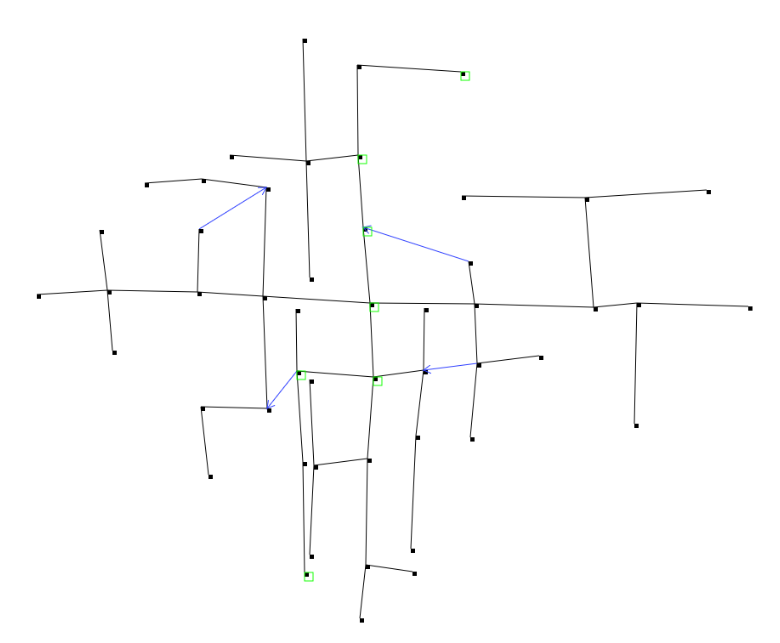
\includegraphics[width=\linewidth]{graph.png}
\caption{Kép a generáló algoritmus eddigi eredményéről}
\label{fig:graph}
\end{figure}
Ezek után következik az utak sávszámának kiadása, az egyirányú utak elhelyezése, valamint a buszmegállók és kanyarok generálása.